% !TEX root = ../CedricDe Schepper2023_Thesis.tex

\section{Related Work}\label{sec:related-work}

This section will detail different types of algorithms researched to solve the timetabling problem.

\begin{description}
    \item [Integer programming] Integer programming tries to solve an optimisation by minimising or maximising the problem's objective function. Fundamentally, some or all required variables are constrained to integers. Since integer programming makes use of an exhaustive search process, the search space must be reduced as much as possible to reduce the run time.
    \item [Simulated Annealing] Simulated Annealing\cite{kirkpatrick1983} makes use of a temperature variable which describes the level of randomness present in the acceptance of a new solution. After generating an initial solution, newly obtained solutions are accepted based on the change in objective function and current temperature. Over time the temperature cools down which reduces the amount of randomness.
    \item [Adaptive Large Neighbourhood Search] Adaptive Large Neighbourhood Search (ALNS) \cite{ropke2006} works by generating new solutions by constantly making changes to the current solution in order to explore the neighbourhood space. These changes are obtained by removing part of the variables and then reintroducing new values in order to generate neighbours. ALNS is considered adaptive since it keeps track of the performance of certain operations and adjusts its parameters accordingly. The use of ALNS for exam timetabling so far has been limited.
    \item [Genetic Algorithms] Genetic Algorithms (GA) \cite{Holland1975} are based on the process of natural selection witnessed in nature. They work by generating an initial set or population of possible solutions. Iteratively, a new population will be formed by selecting the fittest (best) solutions and combining two solutions to create a new generation of solutions.
    \item [Particle Swarm Optimisation] Particle Swarm Optimisation (PSO) \cite{kennedy1995} is derived from the behaviour by collective species as seen in fish schools and bird flocks. A swarm of particles (see fish or bird), representing solutions, moves through the search space at a certain speed and direction.
    \item [Honey-Bee Mating Optimisation] Honey-Bee Mating Optimisation algorithms (HBMO) \cite{abbas2001} are based on the mating of honey-bees as witnessed in nature. During the mating procedure, the queen representing the current best solution is able to mate with other bees in order to produce new solutions.


\end{description}

\subsection{Integer programming}

Kristiansen et al. \cite{kristiansen2015} describes a mixed-integer linear programming (MIP) model designed to solve XHSTT timetabling data sets. The XHSTT format was formulated to standardise timetabling data sets in order to compare heuristics. The proposed model makes use of two stages. During the first stage, a simplified MIP model is generated taking only the hard constraints of the problem into account. This stage is ran until a specified amount of time has passed or until the model has been solved to optimality. The benefit of using integer programming here is that MIP models can issue 'certificates of optimality, indicating that an optimal solution has been reached. This differs from heuristic methods where a model cannot guarantee that an optimal solution has been found unless the objective function is brought to 0. With MIP models, one can determine whether the cost generated by the hard constraints is the most optimal solution feasible. This allows a clear cut off point for the model to stop focusing on the hard constraints solely. 

If a certificate of optimality can be generated, the second stage is executed. Otherwise, the algorithm ends. Before solving the model in stage 2, the soft constraints are added again. Additionally, an extra constraint is added which keeps the optimal value of the cost generated by the hard constraints. The second stage ends after the remaining time after stage 1 has passed. The proposed model was not only successful in creating 2 new solutions to XHSTT data sets, it was also able to prove optimality of previously found solutions. Additionally, it could also provide the lower bounds for several other data sets and improve the best solution found so far. These lower bounds are crucial in order to compare the quality of solutions that have not reached optimality.

Al-hawari et al. \cite{hawari2017} attempts to solve the university exam timetabling problem by splitting the problem into three smaller sub-problems in order to significantly decrease the amount of variables required in the formulas used and thus reduce the processing power and storage capacity needed. Additionally, the simplification of the formulas also improves the explainability of the model, making it easier to understand. The initial problem is split into 3 problems, each sub-problem continuing on the solution provided by the previous phase. Phase one and two will use a  graph colouring IP model to generate a feasible solution. Graph colouring works by assigning colours to the vertices while avoiding that two vertices connected by an edge are assigned the same colour. These vertices are called adjacent. Additionally, graph colouring will attempt to use the least amount of colours possible to generate a feasible solutions.

The first phase starts by assigning time slots to the different exams. Here, exams are seen as the vertices with two vertices being connected by an edge if a student is enrolled in both exams. The time slots act as colours and are assigned to the vertices. Every feasible solution produced by this phase will satisfy the hard constraint that a student can not have more than one exam at the same time. Phase two builds upon this solution by assigning days to the time slots, meaning that the time slots are now considered vertices and the different days colours. Again, vertices are adjacent if the exams assigned to the time slots share mutual students. The new solution will have added the extra constraint that a student can't have two exams on the same day. Lastly, the third stage will assign all exams to rooms, keeping into account the exam enrolment and room capacity. The final solution, if feasible, will satisfy all hard constraints. An important remark to note is that no soft constraints were introduced for creating an improved exam distribution. As a result, a feasible solution will only make sure that a student has no exams on two following days or on the same day.


\subsection{Simulated Annealing}

Aycan and Ayav \cite{aycan2009} apply Simulated Annealing in order to generate optimal solutions. In order to create a initial solution as optimal as possible, constraint satisfaction methods are used to create a solution satisfying all hard constraints. During the simulated annealing phase, a new solution is found by randomly swapping two variables. The cost of the new solution is then calculated using the objective function. Whenever the new objective is lower than the objective of the of the previous solution, the algorithm will keep the new solution. In the case of a higher objective, the temperature will determine based on the difference between the two costs whether to keep the new solution or discard it. The possibility of accepting worsening solutions allows the algorithm to avoid being stuck in local minima. Over time the temperature will reduce based on the cooling schedule. Practically, the allowed difference in cost for worsening solutions in order to still be accepted will decrease. As the temperature decreases, the focus switches from exploring to exploiting the search space. This will allow the algorithm to eventually converge towards a local or global minimum. The performance of Simulated Annealing is determined by the choice of initial solution, the objective function, and cooling schedule. 

The objective function accounts for the impact of both hard as well as soft constraints. Every constraint is assigned its own penalty function including a constraint weight. The cooling schedule proposed makes use of geometric schedule. That means that the temperature will decrease by a constant factor during every step of the algorithm. The choice for the initial temperature and cool-down factor will determine the share of the search space visited. 

While geometric cooling is a very simple to implement, it comes with some shortcoming. Since the temperature is calculated by a deterministic schedule, it mostly depends on the variables chosen by the user. Additionally, this schedule also does not take into account the progress made by the algorithm. Alternative, the more complex adaptive cooling schedules will decrease, or even increase, the temperature based on the rate of acceptance for new solutions. While Aycan and Ayav conclude that this method succeeds in satisfying the hard constraint in order to find a feasible solution, implementing a hybrid version or adding reheating to the cooling schedule might obtain higher quality results.

A more complex cooling schedule can be seen in the Simulated Annealing with Reheating (SAR) algorithm by Leng Goh et al.\cite{Goh2017} They propose a two stage hybrid timetabling algorithm where the first stage uses Tabu search to generate a feasible solution. If such a solution is found, the second stage attempts to improve on it by using SAR. Instead of using geometric cooling, reheating or increasing the temperature is possible. This is based on the assumption that whenever the objective is high, the focus should be on exploration and accordingly whenever the objective is low, exploitation is prioritised. Whenever the search is estimated to be stuck in a local optima, the temperature will be reheated until it manages to escape. 

This estimate is made by checking the difference between the best and current objective. If the change in objective is under a certain threshold for a pre-determined amount of iterations, the search is considered to be stuck and reheating will occur. This cooling and reheating repeats itself until an optimal solution has been found or a step limit is reached. An additional benefit to reheating compared to a geometric schedule is that no fine-tuning of variables is needed when extending the runtime. Figure \ref{fig:SAR} showcases the effect that enabling reheating has on the temperature, with its value increasing whenever it gets stuck in a local optimum. As a consequence, the search is allowed to explore more, resulting in a higher amount of variation of the objective. In this case, the reheating allowed the search to discover a more optimal solution.

\begin{figure}[h]
  \centering
  \subfloat[SAR with reheating disabled]{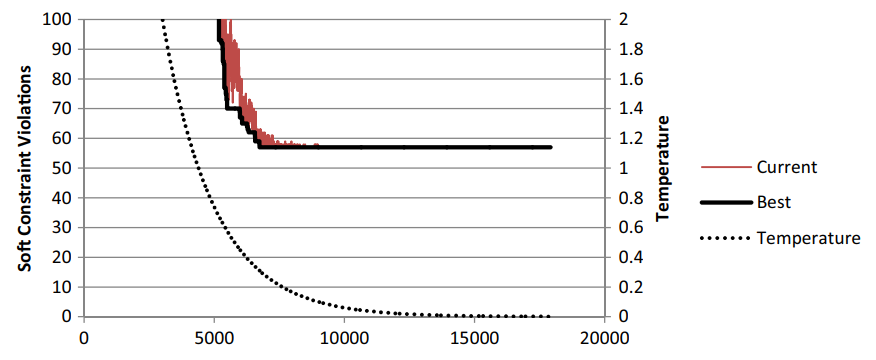
\includegraphics[width=0.5\textwidth]{images/related_works/SA/SAR_disabled.png}}
  \hfill
  \subfloat[SAR with reheating enabled]{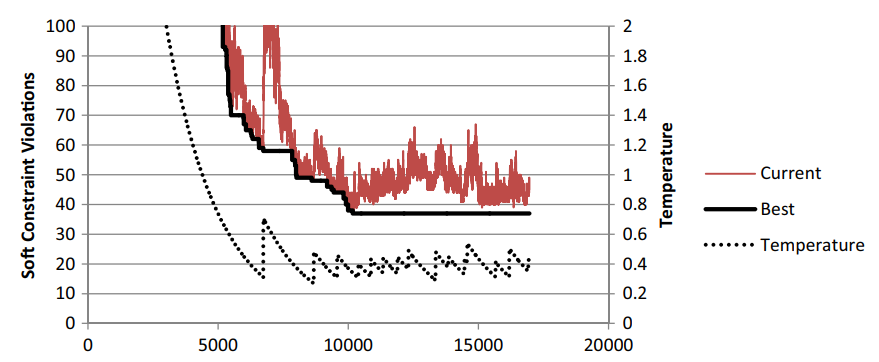
\includegraphics[width=0.5\textwidth]{images/related_works/SA/SAR_enabled.png}}
  \caption{Effect of reheating on the temperate and objective}
  \label{fig:SAR}
\end{figure}

\subsection{Adaptive Large Neighbourhood Search}

S{\o}rensen and Stidsen \cite{sorensen2012} propose a version of ALNS building on the more general Large Neighbourhood Search algorithm. LNS works by creating new solutions by applying a "destroy" and "repair" operation. Every step a destroy operation will remove a set of variables from the problem, before reintroducing new variables in order to create new solutions. By changing multiple variables, LNS is able to escape local minima. In the proposed ALNS extension however, the single destroy and repair operations are replaced by multiple operations, chosen at random during execution. This changes the original deterministic model into a stochastic version, introducing randomness. Additionally an adaptive layer analyses the impact of each operator and increases the probability of operators having a positive impact on the objective function.

\subsection{Genetic Algorithms}

Genetic Algorithms (GA) are based on the process of natural selection witnessed in nature. It generally consists of several base steps before reaching a final solution. Firstly, the algorithm creates an initial population consisting of feasible solutions. An iterative approach is then taken in order to evolve this population into new generations. For every generation, the fitness of each individual in the population is determined and the 'fittest' individuals are chosen as parents for the new generation. In order to obtain new offspring, genetic operators such as crossover and mutation are applied. Crossover works by combining information of parent solutions into a new offspring. This can be done by swapping exam assignments across the parents. Mutation on the other hand randomly changes assignments in order to create new offspring. This is done in order to maintain randomness, allowing GA to escape local minima. The iterative flow of genetic algorithms can be seen in figure \ref{fig:GA}.

\begin{figure}[h]
	\centering
	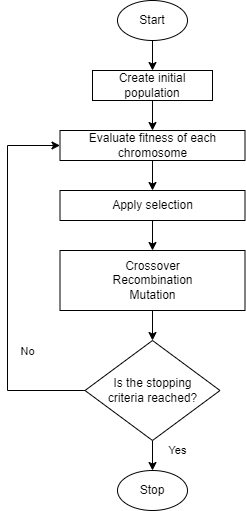
\includegraphics[width=0.35\textwidth]{images/related_works/GA/GA.png} 
	\caption{Iterative approach by genetic algorithms}
	\label{fig:GA}
\end{figure}

% TODO: add GA drawing (GA.drawio)

The paper submitted by Pillay and Banzhaf \cite{pillay2010} showcases a two-phased approach to create feasible timetables. Both phases utilise a genetic algorithm in order to come to a solution, with the first phase focusing on producing a timetable that does not violate any hard constraints. The second phase later attempts the optimise the objective of the soft constraints. Up until 2007, most papers applying genetic algorithms used data sets specific to a particular institution. This algorithm is tested on the Carter benchmarks, allowing its performance to be compared to different approaches.

During the first phase, domain specific heuristics are used instead of random operations in order to create the initial population. While these heuristics requires domain knowledge, the quality of the initial population should be superior. In order to determine the next exam to be assigned, the obtained heuristics make use of the number of conflicts, the number of students enrolled per exam, or the number of students with conflicts. These heuristics were then compared to random and best-slot scheduling. It was found that using heuristics succeeded in lowering the soft constraints objective compared to other scheduling methods. For the iterative steps, the fitness function is described as the amount of conflicts per timetable. In order to select the parents with which to generate the new generation, tournament selection is applied. Here, a determined amount of individuals are randomly chosen from the population to be compared against each other. The individual having the lowest objective ends up being selected. This process is repeated until until all parents have been selected. When creating new offspring, both mutation and crossover operators were considered. During mutation, a random amount of conflicting examinations are rescheduled. Moreover, crossover operations that randomly swap time slots between two parents were tested. This requires an additional repair mechanism to remove duplicate examinations and schedule missing examinations. Since the crossover operations did not have a positive impact on the performance, only mutation was used.

The second phase focuses on minimising the objective of the soft constraints in order the generate a more optimal timetable. While very similar to the first phase,  mutation operations are now continuously applied until an offspring superior to the parent is found or until a certain amount of iterations has been reached. The performance of this genetic algorithm was eventually compared to other studies using the same benchmark including Tabu search and large neighbourhood search. While no optimal solutions were found for any of the data sets, equal or improved solutions were obtained compared to alternative methods.

Chu and Fang \cite{Chu2000} made a comparison between using genetic algorithms versus Tabu search to obtain time tables. For all of their different experiments, the Tabu search implementation was able to outperform their genetic algorithm both on the quality of the solution as the computational time needed to converge. However, a redeeming quality of Tabu search is that it is able to produce several near optimal solutions in one go while Tabu search is limited to a single solution.
\subsection{Particle Swarm Optimisation}

Chen and Shih \cite{Chen2013} discuss a particle swarm optimisation implementation combined with local search %TODO expand on this
During PSO, a swarm of particles, corresponding to different timetables, moves through the available search space. During every iteration, each particle will remember its best encountered position and share its information with the rest of the swarm. The particles will then adjust their velocity and direction on both their personal and global best. The velocity can be seen as the magnitude of the allowed change per time step. In order to avoid particles being trapped in a local optima, an iteration of local search is executed after a particle move. This step will check the surrounding areas for a better solution. 

Tassopoulos and Beligiannis \cite{Tassopoulos2012} builds on the general Particle swarm optimisation algorithm. Initially, they start with a high amount of 150 particles. Whenever the fitness value of a produced particle exceeds a certain tolerance value, this particle is set to inactive and will not be used in further steps. This tolerance value is calculated during each step in order to deactivate weak particles at the start but make it harder for particles to reach that threshold down the line. When the amount of particles is reduced to 30, this procedure stops. The reasoning behind starting with a large amount of particles is to make it possible to explore a wider search space while keeping the execution time down by reducing the particles over time. Similar to Chen and Shih's approach \cite{Chen2013} a local search algorithm is used to minimise one of the soft constraints. Results show that it outperforms the genetic and evolutionary algorithms that the particle swarm optimisation implementation was tested against.
\subsection{Honey-Bee Mating Optimisation}

Sabar et al. \cite{Sabar2009} are the first to propose the use of Honey-bee mating optimisation in order to solve the exam timetabling problem. Since specific terms used in the natural mating process are used when describing the optimisation algorithm, table \ref{tab:hbmo} provides translation of the analogy. The original HBMO algorithm starts follows the natural process when the queen leaves the hive on a mating flight. Here she maintains a certain speed and direction, creating the possibility of drones to mate with her. After mating with a drone, its genetic information is stored within the queen to be used in the breeding phase. After each mating, the queen will change her energy and speed. As soon as the queen reaches a certain energy threshold or reaches a mating limit, she will return to the hive. Upon return, the queen will randomly select genetic information obtained and perform a crossover step to create a new brood. Every brood is fed by a worker in order to improve the obtained solution. After every brood is improved, the fittest brood is compared to the queen. If the brood corresponds to a superior solution, the queen is replaced by the brood. Both the queen and the other broods are killed and a new mating flight will commence. 

The variant on the original HBMO algorithm proposed by Sabar et al. attempts to solve HBMO's weakness of suffering from early convergence. In the original algorithm, the drones used to mate with the queen are never replaced which reduces the amount of variation. This is solved by replacing the drones that were successful in mating with the newly created broods. Additionally, after crossover, the heuristic applied by the worker is based on local search in order to optimise the brood as much as possible.

While HBMO is very similar to other population based methods such as genetic algorithms, two clear differences can be noted. HBMO maintains the queen as one of the two 'parents' used during crossover. Since the queen is considered as the current best solution, this is meant to improve obtained solutions. Secondly, the local search applied by the worker can be considered an exploitation phase which is not present in genetic algorithms. Finally, they conclude that the proposed HBMO alternative manages to create comparable or superior solutions compared against other population based methods.

\begin{table}[h]
	\caption{Analogy between the natural mating process and the HBMO algorithm}
	\label{tab:hbmo}
	\centering
	\begin{tabular}{l c c }
		\hline
		\textbf{Natural honey bee}  & \textbf{Artificial honey bee} \\ \hline
		Queen & Current best solution \\
		Drones & Possible solutions \\
	    Broods & Newly generated solutions \\
            Worker & Heuristic search \\
            Mating or Breeding & Crossover \\ \hline
	\end{tabular}
\end{table}


